\documentclass{article}\usepackage[]{graphicx}\usepackage[]{color}
%% maxwidth is the original width if it is less than linewidth
%% otherwise use linewidth (to make sure the graphics do not exceed the margin)
\makeatletter
\def\maxwidth{ %
  \ifdim\Gin@nat@width>\linewidth
    \linewidth
  \else
    \Gin@nat@width
  \fi
}
\makeatother

\definecolor{fgcolor}{rgb}{0.345, 0.345, 0.345}
\newcommand{\hlnum}[1]{\textcolor[rgb]{0.686,0.059,0.569}{#1}}%
\newcommand{\hlstr}[1]{\textcolor[rgb]{0.192,0.494,0.8}{#1}}%
\newcommand{\hlcom}[1]{\textcolor[rgb]{0.678,0.584,0.686}{\textit{#1}}}%
\newcommand{\hlopt}[1]{\textcolor[rgb]{0,0,0}{#1}}%
\newcommand{\hlstd}[1]{\textcolor[rgb]{0.345,0.345,0.345}{#1}}%
\newcommand{\hlkwa}[1]{\textcolor[rgb]{0.161,0.373,0.58}{\textbf{#1}}}%
\newcommand{\hlkwb}[1]{\textcolor[rgb]{0.69,0.353,0.396}{#1}}%
\newcommand{\hlkwc}[1]{\textcolor[rgb]{0.333,0.667,0.333}{#1}}%
\newcommand{\hlkwd}[1]{\textcolor[rgb]{0.737,0.353,0.396}{\textbf{#1}}}%
\let\hlipl\hlkwb

\usepackage{framed}
\makeatletter
\newenvironment{kframe}{%
 \def\at@end@of@kframe{}%
 \ifinner\ifhmode%
  \def\at@end@of@kframe{\end{minipage}}%
  \begin{minipage}{\columnwidth}%
 \fi\fi%
 \def\FrameCommand##1{\hskip\@totalleftmargin \hskip-\fboxsep
 \colorbox{shadecolor}{##1}\hskip-\fboxsep
     % There is no \\@totalrightmargin, so:
     \hskip-\linewidth \hskip-\@totalleftmargin \hskip\columnwidth}%
 \MakeFramed {\advance\hsize-\width
   \@totalleftmargin\z@ \linewidth\hsize
   \@setminipage}}%
 {\par\unskip\endMakeFramed%
 \at@end@of@kframe}
\makeatother

\definecolor{shadecolor}{rgb}{.97, .97, .97}
\definecolor{messagecolor}{rgb}{0, 0, 0}
\definecolor{warningcolor}{rgb}{1, 0, 1}
\definecolor{errorcolor}{rgb}{1, 0, 0}
\newenvironment{knitrout}{}{} % an empty environment to be redefined in TeX

\usepackage{alltt}
\usepackage[margin=3cm]{geometry}
\IfFileExists{upquote.sty}{\usepackage{upquote}}{}
\begin{document}



\title{curatedMetagenomicData Data Application - Scenario 1}
\date{}
\maketitle

Load packages.
\begin{knitrout}
\definecolor{shadecolor}{rgb}{0.969, 0.969, 0.969}\color{fgcolor}\begin{kframe}
\begin{alltt}
\hlkwd{library}\hlstd{(curatedMetagenomicData)}
\hlkwd{library}\hlstd{(plyr)}
\hlkwd{library}\hlstd{(FSelector)}
\hlkwd{library}\hlstd{(glmnet)}
\hlkwd{library}\hlstd{(data.table)}
\hlkwd{library}\hlstd{(nlme)}
\hlkwd{library}\hlstd{(lme4)}
\end{alltt}
\end{kframe}
\end{knitrout}

Load data.
\begin{knitrout}
\definecolor{shadecolor}{rgb}{0.969, 0.969, 0.969}\color{fgcolor}\begin{kframe}
\begin{alltt}
\hlstd{metadata} \hlkwb{=} \hlkwd{curatedMetagenomicData}\hlstd{(}\hlstr{"QinJ_2012.marker_abundance.stool"}\hlstd{,} \hlkwc{dryrun} \hlstd{=} \hlnum{FALSE}\hlstd{)}
\hlstd{meta.merged} \hlkwb{=} \hlkwd{mergeData}\hlstd{(metadata)}
\hlkwd{rm}\hlstd{(}\hlkwc{list}\hlstd{=}\hlkwd{c}\hlstd{(}\hlstr{"metadata"}\hlstd{))}
\end{alltt}
\end{kframe}
\end{knitrout}

Add clinical variables to marker abundance data and restrict to female patients.
\begin{knitrout}
\definecolor{shadecolor}{rgb}{0.969, 0.969, 0.969}\color{fgcolor}\begin{kframe}
\begin{alltt}
\hlstd{meta.exp} \hlkwb{=} \hlkwd{data.frame}\hlstd{(}\hlkwd{t}\hlstd{(}\hlkwd{exprs}\hlstd{(meta.merged)))}
\hlstd{meta.exp}\hlopt{$}\hlstd{cholesterol} \hlkwb{=} \hlstd{meta.merged}\hlopt{$}\hlstd{cholesterol}
\hlstd{meta.exp}\hlopt{$}\hlstd{age} \hlkwb{=} \hlstd{meta.merged}\hlopt{$}\hlstd{age}
\hlstd{meta.exp} \hlkwb{=} \hlstd{meta.exp[}\hlkwd{which}\hlstd{(meta.merged}\hlopt{$}\hlstd{gender}\hlopt{==}\hlstr{"female"}\hlstd{),]}
\hlstd{meta.exp} \hlkwb{=} \hlstd{meta.exp[}\hlkwd{complete.cases}\hlstd{(meta.exp),]}
\end{alltt}
\end{kframe}
\end{knitrout}

Divide dataset into training and test sets.
\begin{knitrout}
\definecolor{shadecolor}{rgb}{0.969, 0.969, 0.969}\color{fgcolor}\begin{kframe}
\begin{alltt}
\hlkwd{set.seed}\hlstd{(}\hlnum{123}\hlstd{)}
\hlcom{# number of training datasets}
\hlstd{ndat} \hlkwb{=} \hlnum{4}
\hlstd{ind.train} \hlkwb{=} \hlkwd{sample}\hlstd{(}\hlnum{1}\hlopt{:}\hlkwd{nrow}\hlstd{(meta.exp),} \hlkwd{ceiling}\hlstd{(}\hlkwd{nrow}\hlstd{(meta.exp)}\hlopt{*}\hlstd{(ndat)}\hlopt{/}\hlstd{(ndat}\hlopt{+}\hlnum{1}\hlstd{)))}
\hlstd{qin.train} \hlkwb{=} \hlstd{meta.exp[ind.train,]}
\hlstd{qin.test} \hlkwb{=} \hlstd{meta.exp[}\hlopt{-}\hlstd{ind.train,]}
\hlstd{qin.train}\hlopt{$}\hlstd{group} \hlkwb{=} \hlkwd{sample}\hlstd{(}\hlnum{1}\hlopt{:}\hlstd{ndat,} \hlkwd{nrow}\hlstd{(qin.train),} \hlkwc{replace}\hlstd{=T)}
\hlstd{qin.test}\hlopt{$}\hlstd{group} \hlkwb{=} \hlstd{ndat}\hlopt{+}\hlnum{1}
\hlstd{group} \hlkwb{=} \hlstd{qin.train}\hlopt{$}\hlstd{group}
\end{alltt}
\end{kframe}
\end{knitrout}

Use the top 5 marker abundances most highly correlated with the outcome in the training set as the predictors.
\begin{knitrout}
\definecolor{shadecolor}{rgb}{0.969, 0.969, 0.969}\color{fgcolor}\begin{kframe}
\begin{alltt}
\hlstd{qin.train} \hlkwb{=} \hlstd{qin.train[,} \hlkwd{which}\hlstd{(}\hlkwd{colSums}\hlstd{(qin.train)}\hlopt{!=}\hlnum{0}\hlstd{)]}

\hlcom{# remove features that are very sparse in the training data}
\hlstd{min.samples} \hlkwb{=} \hlnum{4}
\hlstd{qin.train} \hlkwb{=} \hlstd{qin.train[}\hlkwd{vapply}\hlstd{(qin.train,}
                             \hlkwa{function}\hlstd{(}\hlkwc{x}\hlstd{)} \hlkwd{length}\hlstd{(}\hlkwd{unique}\hlstd{(x))}\hlopt{>}\hlstd{min.samples,} \hlkwd{logical}\hlstd{(}\hlnum{1L}\hlstd{))]}

\hlcom{# calculate correlation for each feature}
\hlstd{feature.list} \hlkwb{=} \hlkwd{lapply}\hlstd{(}\hlkwd{split}\hlstd{(}\hlkwd{as.list}\hlstd{(}\hlkwd{as.data.frame}\hlstd{(qin.train[,} \hlkwd{which}\hlstd{(}\hlopt{!}\hlkwd{names}\hlstd{(qin.train)} \hlopt
                                                                      \hlkwd{c}\hlstd{(}\hlstr{"cholesterol"}\hlstd{,} \hlstr{"age"}\hlstd{))])),}
                            \hlkwd{cut}\hlstd{(}\hlnum{1}\hlopt{:}\hlkwd{ncol}\hlstd{(qin.train[,} \hlkwd{which}\hlstd{(}\hlopt{!}\hlkwd{names}\hlstd{(qin.train)} \hlopt
                                                           \hlkwd{c}\hlstd{(}\hlstr{"cholesterol"}\hlstd{,} \hlstr{"age"}\hlstd{))]),} \hlnum{20}\hlstd{)),}
                      \hlstd{as.data.frame)}
\hlstd{weight.list} \hlkwb{=} \hlkwd{lapply}\hlstd{(feature.list,} \hlkwa{function}\hlstd{(}\hlkwc{x}\hlstd{)} \hlkwd{linear.correlation}\hlstd{(qin.train}\hlopt{$}\hlstd{cholesterol} \hlopt{~}\hlstd{., x))}
\hlstd{weight.df} \hlkwb{=} \hlkwd{rbind.fill}\hlstd{(weight.list)}
\hlstd{weight.df}\hlopt{$}\hlstd{feature} \hlkwb{=} \hlkwd{unlist}\hlstd{(}\hlkwd{lapply}\hlstd{(weight.list, row.names))}
\hlstd{weight.df} \hlkwb{=} \hlstd{weight.df[}\hlkwd{order}\hlstd{(weight.df}\hlopt{$}\hlstd{attr_importance,} \hlkwc{decreasing} \hlstd{= T), ]}
\hlcom{# get top 5 features}
\hlstd{max.features} \hlkwb{=} \hlnum{5}
\hlstd{qin.train} \hlkwb{=} \hlkwd{cbind}\hlstd{(qin.train[,} \hlkwd{which}\hlstd{(}\hlkwd{names}\hlstd{(qin.train)} \hlopt \hlkwd{c}\hlstd{(weight.df}\hlopt{$}\hlstd{feature[}\hlnum{1}\hlopt{:}\hlstd{max.features],}
                                                            \hlkwd{c}\hlstd{(}\hlstr{"cholesterol"}\hlstd{,} \hlstr{"age"}\hlstd{)))], group)}
\hlstd{qin.test} \hlkwb{=} \hlstd{qin.test[,} \hlkwd{which}\hlstd{(}\hlkwd{names}\hlstd{(qin.test)} \hlopt \hlkwd{c}\hlstd{(weight.df}\hlopt{$}\hlstd{feature[}\hlnum{1}\hlopt{:}\hlstd{max.features],}
                                                   \hlkwd{c}\hlstd{(}\hlstr{"cholesterol"}\hlstd{,} \hlstr{"age"}\hlstd{,} \hlstr{"group"}\hlstd{)))]}
\end{alltt}
\end{kframe}
\end{knitrout}

Set up design matrices.
\begin{knitrout}
\definecolor{shadecolor}{rgb}{0.969, 0.969, 0.969}\color{fgcolor}\begin{kframe}
\begin{alltt}
\hlstd{qin.all} \hlkwb{=} \hlkwd{rbind}\hlstd{(qin.train, qin.test)}
\hlstd{parts} \hlkwb{=} \hlkwd{split}\hlstd{(qin.all, qin.all}\hlopt{$}\hlstd{group)}
\hlstd{edat_train} \hlkwb{=} \hlstd{parts[}\hlnum{1}\hlopt{:}\hlstd{ndat]}
\hlstd{edat_test} \hlkwb{=} \hlstd{parts[ndat}\hlopt{+}\hlnum{1}\hlstd{]}
\hlstd{train} \hlkwb{=} \hlkwd{rbindlist}\hlstd{(edat_train)}
\hlstd{test} \hlkwb{=} \hlkwd{rbindlist}\hlstd{(edat_test)}
\end{alltt}
\end{kframe}
\end{knitrout}

Estimate random effect variances and variance of residuals using REML via a linear mixed effects model.
\begin{knitrout}
\definecolor{shadecolor}{rgb}{0.969, 0.969, 0.969}\color{fgcolor}\begin{kframe}
\begin{alltt}
\hlstd{features} \hlkwb{=} \hlkwd{names}\hlstd{(train)[}\hlkwd{which}\hlstd{(}\hlopt{!}\hlkwd{names}\hlstd{(train)} \hlopt \hlkwd{c}\hlstd{(}\hlstr{"cholesterol"}\hlstd{,} \hlstr{"group"}\hlstd{))]}
\hlstd{lm.formula} \hlkwb{=} \hlkwd{as.formula}\hlstd{(}\hlkwd{paste}\hlstd{(}\hlstr{"cholesterol~"}\hlstd{,} \hlkwd{paste0}\hlstd{(features,} \hlkwc{collapse}\hlstd{=}\hlstr{"+"}\hlstd{)))}
\hlstd{feature.cols} \hlkwb{=} \hlkwd{which}\hlstd{(}\hlkwd{names}\hlstd{(train)} \hlopt \hlkwd{c}\hlstd{(features))}

\hlstd{lmer.formula} \hlkwb{=} \hlkwd{as.formula}\hlstd{(}\hlkwd{paste}\hlstd{(}\hlstr{"cholesterol~ (1|group) +"}\hlstd{,}
                                \hlkwd{paste0}\hlstd{(}\hlkwd{unique}\hlstd{(}\hlkwd{names}\hlstd{(train)[feature.cols]),} \hlkwc{collapse}\hlstd{=}\hlstr{"+"}\hlstd{),} \hlstr{"+"}\hlstd{,}
                                \hlkwd{paste0}\hlstd{(}\hlstr{"(0+"}\hlstd{,} \hlkwd{names}\hlstd{(train)[feature.cols],} \hlstr{"|group)"}\hlstd{,} \hlkwc{collapse}\hlstd{=}\hlstr{"+"}\hlstd{)))}
\hlstd{tol} \hlkwb{=} \hlnum{1e-10}
\hlstd{fit.lmer} \hlkwb{=} \hlkwd{lmer}\hlstd{(lmer.formula,} \hlkwc{data}\hlstd{=train)}
\hlstd{ind.re} \hlkwb{=} \hlkwd{which}\hlstd{(}\hlkwd{as.data.frame}\hlstd{(}\hlkwd{VarCorr}\hlstd{(fit.lmer))[}\hlnum{2}\hlopt{:}\hlstd{(}\hlkwd{length}\hlstd{(feature.cols)}\hlopt{+}\hlnum{1}\hlstd{),} \hlnum{4}\hlstd{]}\hlopt{>}\hlstd{tol)}
\hlstd{sigma.eps} \hlkwb{=} \hlkwd{summary}\hlstd{(fit.lmer)}\hlopt{$}\hlstd{sigma}
\hlkwd{as.data.frame}\hlstd{(}\hlkwd{VarCorr}\hlstd{(fit.lmer))[}\hlnum{1}\hlopt{:}\hlstd{(}\hlkwd{length}\hlstd{(feature.cols)}\hlopt{+}\hlnum{1}\hlstd{),} \hlnum{4}\hlstd{]}
\end{alltt}
\begin{verbatim}
## [1] 3.292003e-05 5.073568e-05 0.000000e+00 0.000000e+00 6.950433e-05
## [6] 0.000000e+00 0.000000e+00
\end{verbatim}
\begin{alltt}
\hlstd{sigma2.bar} \hlkwb{=} \hlkwd{mean}\hlstd{(}\hlkwd{as.data.frame}\hlstd{(}\hlkwd{VarCorr}\hlstd{(fit.lmer))[}\hlnum{1}\hlopt{:}\hlstd{(}\hlkwd{length}\hlstd{(feature.cols)}\hlopt{+}\hlnum{1}\hlstd{),} \hlnum{4}\hlstd{])}
\hlstd{sigma2.bar}
\end{alltt}
\begin{verbatim}
## [1] 2.188001e-05
\end{verbatim}
\end{kframe}
\end{knitrout}


Estimate optimal LS weights.
\begin{knitrout}
\definecolor{shadecolor}{rgb}{0.969, 0.969, 0.969}\color{fgcolor}\begin{kframe}
\begin{alltt}
\hlkwd{source}\hlstd{(}\hlstr{"../simulations/transition_point_fns.R"}\hlstd{)}
\hlstd{parts2} \hlkwb{=} \hlkwd{split}\hlstd{(}\hlkwd{cbind}\hlstd{(}\hlkwd{rep}\hlstd{(}\hlnum{1}\hlstd{,} \hlkwd{nrow}\hlstd{(qin.all)), qin.all[, feature.cols]),}
               \hlstd{qin.all}\hlopt{$}\hlstd{group)}
\hlstd{edat_train2} \hlkwb{=} \hlstd{parts2[}\hlnum{1}\hlopt{:}\hlstd{ndat]}
\hlstd{edat_test2} \hlkwb{=} \hlstd{parts2[ndat}\hlopt{+}\hlnum{1}\hlstd{]}

\hlcom{# estimate optimal LS weights}
\hlstd{vec.re} \hlkwb{=} \hlkwd{sqrt}\hlstd{(}\hlkwd{as.data.frame}\hlstd{(}\hlkwd{VarCorr}\hlstd{(fit.lmer))[}\hlnum{1}\hlopt{:}\hlstd{(}\hlkwd{length}\hlstd{(feature.cols)}\hlopt{+}\hlnum{1}\hlstd{),} \hlnum{4}\hlstd{])}
\hlstd{wk.ols} \hlkwb{=} \hlkwd{optimal_weights}\hlstd{(edat_train2, edat_test2, sigma.eps, vec.re)}
\hlstd{wk.ols}
\end{alltt}
\begin{verbatim}
## [1] 0.454403415 0.304337930 0.231621326 0.009637329
\end{verbatim}
\end{kframe}
\end{knitrout}

Tune ridge regression regularization parameters. 
\begin{knitrout}
\definecolor{shadecolor}{rgb}{0.969, 0.969, 0.969}\color{fgcolor}\begin{kframe}
\begin{alltt}
\hlcom{# choose regularization parameter}
\hlkwd{set.seed}\hlstd{(}\hlnum{1}\hlstd{)}
\hlstd{cv.ridge.merged} \hlkwb{=} \hlkwd{cv.glmnet}\hlstd{(}\hlkwd{data.matrix}\hlstd{(train)[, feature.cols], train}\hlopt{$}\hlstd{cholesterol,}
                            \hlkwc{alpha} \hlstd{=} \hlnum{0}\hlstd{,}
                            \hlkwc{intercept}\hlstd{=T,} \hlkwc{lambda}\hlstd{=}\hlnum{2}\hlopt{^}\hlkwd{seq}\hlstd{(}\hlopt{-}\hlnum{8}\hlstd{,} \hlnum{8}\hlstd{,} \hlkwc{length}\hlstd{=}\hlnum{100}\hlstd{),} \hlkwc{standardize}\hlstd{=F)}
\hlstd{sd.y} \hlkwb{=} \hlkwd{sqrt}\hlstd{(}\hlkwd{var}\hlstd{(train}\hlopt{$}\hlstd{cholesterol)}\hlopt{*}\hlstd{(}\hlkwd{length}\hlstd{(train}\hlopt{$}\hlstd{cholesterol)}\hlopt{-}\hlnum{1}\hlstd{)}\hlopt{/}\hlkwd{length}\hlstd{(train}\hlopt{$}\hlstd{cholesterol))}
\hlcom{# compute regularization parameter for formulation of ridge regression objective function assumed by transition_point_fns.R (https://stats.stackexchange.com/questions/129179/why-is-glmnet-ridge-regression-giving-me-a-different-answer-than-manual-calculat)}
\hlstd{lam} \hlkwb{=} \hlstd{cv.ridge.merged}\hlopt{$}\hlstd{lambda.min}\hlopt{*}\hlkwd{nrow}\hlstd{(train)}\hlopt{/}\hlstd{sd.y}

\hlstd{lamk} \hlkwb{=} \hlkwd{rep}\hlstd{(}\hlnum{NA}\hlstd{, ndat)}

\hlkwa{for} \hlstd{(i} \hlkwa{in} \hlnum{1}\hlopt{:}\hlstd{ndat) \{}
  \hlstd{dataset} \hlkwb{=} \hlstd{edat_train[[i]]}

  \hlkwd{set.seed}\hlstd{(}\hlnum{1}\hlstd{)}
  \hlstd{cv.ridge} \hlkwb{=} \hlkwd{cv.glmnet}\hlstd{(}\hlkwd{data.matrix}\hlstd{(dataset)[, feature.cols], dataset}\hlopt{$}\hlstd{cholesterol,}
                       \hlkwc{alpha} \hlstd{=} \hlnum{0}\hlstd{,}
                       \hlkwc{intercept}\hlstd{=T,} \hlkwc{lambda}\hlstd{=}\hlnum{2}\hlopt{^}\hlkwd{seq}\hlstd{(}\hlopt{-}\hlnum{8}\hlstd{,} \hlnum{8}\hlstd{,} \hlkwc{length}\hlstd{=}\hlnum{100}\hlstd{),}
                       \hlkwc{standardize}\hlstd{=F,} \hlkwc{nfolds}\hlstd{=}\hlnum{5}\hlstd{)}
  \hlstd{sd.y} \hlkwb{=} \hlkwd{sqrt}\hlstd{(}\hlkwd{var}\hlstd{(dataset}\hlopt{$}\hlstd{cholesterol)}\hlopt{*}\hlstd{(}\hlkwd{length}\hlstd{(dataset}\hlopt{$}\hlstd{cholesterol)}\hlopt{-}\hlnum{1}\hlstd{)}\hlopt{/}\hlkwd{length}\hlstd{(dataset}\hlopt{$}\hlstd{cholesterol))}
  \hlstd{lamk[i]} \hlkwb{=} \hlstd{cv.ridge}\hlopt{$}\hlstd{lambda.min}\hlopt{*}\hlkwd{nrow}\hlstd{(dataset)}\hlopt{/}\hlstd{sd.y}
\hlstd{\}}
\end{alltt}
\end{kframe}
\end{knitrout}


Train and validate merged LS model. 
\begin{knitrout}
\definecolor{shadecolor}{rgb}{0.969, 0.969, 0.969}\color{fgcolor}\begin{kframe}
\begin{alltt}
\hlstd{fit.ols.merged} \hlkwb{=} \hlkwd{lm}\hlstd{(lm.formula,} \hlkwc{data}\hlstd{=train)}
\hlstd{pred.ols.merged} \hlkwb{=} \hlkwd{predict}\hlstd{(fit.ols.merged,} \hlkwc{newdata}\hlstd{=test)}
\hlstd{err.ols.merged} \hlkwb{=} \hlkwd{mean}\hlstd{((pred.ols.merged}\hlopt{-}\hlstd{test}\hlopt{$}\hlstd{cholesterol)}\hlopt{^}\hlnum{2}\hlstd{)}
\hlkwd{sqrt}\hlstd{(err.ols.merged)}
\end{alltt}
\begin{verbatim}
## [1] 53.62371
\end{verbatim}
\end{kframe}
\end{knitrout}


Train and validate merged ridge regression model.
\begin{knitrout}
\definecolor{shadecolor}{rgb}{0.969, 0.969, 0.969}\color{fgcolor}\begin{kframe}
\begin{alltt}
\hlstd{fit.ridge.merged} \hlkwb{=} \hlkwd{glmnet}\hlstd{(}\hlkwd{data.matrix}\hlstd{(train)[, feature.cols], train}\hlopt{$}\hlstd{cholesterol,}
                          \hlkwc{alpha} \hlstd{=} \hlnum{0}\hlstd{,}
                          \hlkwc{lambda} \hlstd{= cv.ridge.merged}\hlopt{$}\hlstd{lambda.min,}
                          \hlkwc{intercept}\hlstd{=T,} \hlkwc{standardize}\hlstd{=F)}
\hlstd{pred.ridge.merged} \hlkwb{=} \hlkwd{predict}\hlstd{(fit.ridge.merged,} \hlkwc{newx}\hlstd{=}\hlkwd{data.matrix}\hlstd{(test)[, feature.cols])}
\hlstd{err.ridge.merged} \hlkwb{=} \hlkwd{mean}\hlstd{((pred.ridge.merged} \hlopt{-} \hlstd{test}\hlopt{$}\hlstd{cholesterol)}\hlopt{^}\hlnum{2}\hlstd{)}
\hlkwd{sqrt}\hlstd{(err.ridge.merged)}
\end{alltt}
\begin{verbatim}
## [1] 59.07932
\end{verbatim}
\end{kframe}
\end{knitrout}

Calculate transition intervals using optimal LS weights for the CSLs.
\begin{knitrout}
\definecolor{shadecolor}{rgb}{0.969, 0.969, 0.969}\color{fgcolor}\begin{kframe}
\begin{alltt}
\hlkwa{if} \hlstd{(}\hlkwd{as.data.frame}\hlstd{(}\hlkwd{VarCorr}\hlstd{(fit.lmer))[}\hlnum{1}\hlstd{,} \hlnum{4}\hlstd{]} \hlopt{>} \hlstd{tol) \{}
  \hlstd{ind.re} \hlkwb{=} \hlkwd{c}\hlstd{(}\hlnum{0}\hlstd{, ind.re)}
\hlstd{\}}

\hlstd{clist} \hlkwb{=} \hlkwd{as.list}\hlstd{(ind.re}\hlopt{+}\hlnum{1}\hlstd{)}

\hlstd{wk.eq} \hlkwb{=} \hlkwd{rep}\hlstd{(}\hlnum{1}\hlstd{, ndat)}\hlopt{/}\hlstd{ndat}

\hlstd{ls.bounds} \hlkwb{=} \hlkwd{tau_ls_range}\hlstd{(edat_train2, edat_test2, wk.eq, sigma.eps,} \hlkwc{cols_re_list}\hlstd{=clist)}
\hlstd{ls.bounds}
\end{alltt}
\begin{verbatim}
## [1] 7.089301e-02 1.373470e+04
\end{verbatim}
\begin{alltt}
\hlstd{ridge.bounds} \hlkwb{=} \hlkwd{tau_r_range}\hlstd{(edat_train2, edat_test2, wk.eq, sigma.eps,} \hlkwc{lambda}\hlstd{=lam,} \hlkwc{lambdak}\hlstd{=lamk,}
                           \hlkwc{beta}\hlstd{=fit.ols.merged}\hlopt{$}\hlstd{coefficients,} \hlkwc{cols_re_list}\hlstd{=clist)}
\hlstd{ridge.bounds}
\end{alltt}
\begin{verbatim}
## [1] 2.449549e-03 6.241744e+02
\end{verbatim}
\begin{alltt}
\hlstd{sigma2.bar} \hlopt{<} \hlstd{ls.bounds[}\hlnum{1}\hlstd{]}
\end{alltt}
\begin{verbatim}
## [1] TRUE
\end{verbatim}
\begin{alltt}
\hlstd{sigma2.bar} \hlopt{<} \hlstd{ridge.bounds[}\hlnum{1}\hlstd{]}
\end{alltt}
\begin{verbatim}
## [1] TRUE
\end{verbatim}
\end{kframe}
\end{knitrout}


Train and validate CSLs.
\begin{knitrout}
\definecolor{shadecolor}{rgb}{0.969, 0.969, 0.969}\color{fgcolor}\begin{kframe}
\begin{alltt}
\hlstd{beta.ols.mat} \hlkwb{=} \hlkwd{matrix}\hlstd{(}\hlkwc{data}\hlstd{=}\hlnum{NA}\hlstd{,} \hlkwc{nrow}\hlstd{=ndat,} \hlkwc{ncol}\hlstd{=}\hlkwd{length}\hlstd{(fit.ols.merged}\hlopt{$}\hlstd{coefficients))}
\hlstd{beta.ols.mat.opt} \hlkwb{=} \hlstd{beta.ols.mat}

\hlstd{beta.ridge.mat} \hlkwb{=} \hlstd{beta.ols.mat}
\hlstd{ols.mat} \hlkwb{=} \hlkwd{matrix}\hlstd{(}\hlkwc{data}\hlstd{=}\hlnum{NA}\hlstd{,} \hlkwc{nrow}\hlstd{=ndat,} \hlkwc{ncol}\hlstd{=}\hlkwd{nrow}\hlstd{(test))}
\hlstd{ridge.mat} \hlkwb{=} \hlstd{ols.mat}

\hlcom{# fit models to each study}
\hlkwa{for} \hlstd{(i} \hlkwa{in} \hlnum{1}\hlopt{:}\hlstd{ndat) \{}

  \hlstd{dataset} \hlkwb{=} \hlstd{edat_train[[i]]}

  \hlcom{# OLS}
  \hlstd{fit.ols} \hlkwb{=} \hlkwd{lm}\hlstd{(lm.formula,} \hlkwc{data}\hlstd{=dataset)}
  \hlstd{beta.ols.mat[i, ]} \hlkwb{=} \hlstd{fit.ols}\hlopt{$}\hlstd{coefficients}
  \hlstd{ols.mat[i, ]} \hlkwb{=} \hlkwd{predict}\hlstd{(fit.ols,} \hlkwc{newdata}\hlstd{=test)}

  \hlcom{# ridge}
  \hlstd{sd.y} \hlkwb{=} \hlkwd{sqrt}\hlstd{(}\hlkwd{var}\hlstd{(dataset}\hlopt{$}\hlstd{cholesterol)}\hlopt{*}\hlstd{(}\hlkwd{length}\hlstd{(dataset}\hlopt{$}\hlstd{cholesterol)}\hlopt{-}\hlnum{1}\hlstd{)}\hlopt{/}\hlkwd{length}\hlstd{(dataset}\hlopt{$}\hlstd{cholesterol))}
  \hlstd{fit.ridge} \hlkwb{=} \hlkwd{glmnet}\hlstd{(}\hlkwd{data.matrix}\hlstd{(dataset)[, feature.cols], dataset}\hlopt{$}\hlstd{cholesterol,}
                     \hlkwc{alpha} \hlstd{=} \hlnum{0}\hlstd{,}
                     \hlkwc{lambda} \hlstd{= lamk[i]}\hlopt{*}\hlstd{sd.y}\hlopt{/}\hlkwd{nrow}\hlstd{(dataset),}
                     \hlkwc{intercept}\hlstd{=T,} \hlkwc{standardize}\hlstd{=F)}
  \hlstd{beta.ridge.mat[i, ]} \hlkwb{=} \hlkwd{c}\hlstd{(fit.ridge}\hlopt{$}\hlstd{a0,} \hlkwd{as.vector}\hlstd{(fit.ridge}\hlopt{$}\hlstd{beta))}
  \hlstd{ridge.mat[i, ]} \hlkwb{=} \hlkwd{predict}\hlstd{(fit.ridge,} \hlkwc{newx}\hlstd{=}\hlkwd{data.matrix}\hlstd{(test)[, feature.cols])}
\hlstd{\}}

\hlstd{pred.ols.csl.eq} \hlkwb{=} \hlstd{wk.eq} \hlopt \hlstd{ols.mat}
\hlstd{err.ols.csl.eq} \hlkwb{=} \hlkwd{mean}\hlstd{((pred.ols.csl.eq}\hlopt{-}\hlstd{test}\hlopt{$}\hlstd{cholesterol)}\hlopt{^}\hlnum{2}\hlstd{)}
\hlkwd{sqrt}\hlstd{(err.ols.csl.eq)}
\end{alltt}
\begin{verbatim}
## [1] 202.1047
\end{verbatim}
\begin{alltt}
\hlstd{pred.ols.csl} \hlkwb{=} \hlstd{wk.ols} \hlopt \hlstd{ols.mat}
\hlstd{err.ols.csl} \hlkwb{=} \hlkwd{mean}\hlstd{((pred.ols.csl}\hlopt{-}\hlstd{test}\hlopt{$}\hlstd{cholesterol)}\hlopt{^}\hlnum{2}\hlstd{)}
\hlkwd{sqrt}\hlstd{(err.ols.csl)}
\end{alltt}
\begin{verbatim}
## [1] 85.69544
\end{verbatim}
\begin{alltt}
\hlstd{pred.ridge.csl.eq} \hlkwb{=} \hlstd{wk.eq} \hlopt \hlstd{ridge.mat}
\hlstd{err.ridge.csl.eq} \hlkwb{=} \hlkwd{mean}\hlstd{((pred.ridge.csl.eq}\hlopt{-}\hlstd{test}\hlopt{$}\hlstd{cholesterol)}\hlopt{^}\hlnum{2}\hlstd{)}
\hlkwd{sqrt}\hlstd{(err.ridge.csl.eq)}
\end{alltt}
\begin{verbatim}
## [1] 69.92978
\end{verbatim}
\begin{alltt}
\hlstd{wk.ridge} \hlkwb{=} \hlkwd{optimal_weights_ridge}\hlstd{(edat_train2, edat_test2, sigma.eps, vec.re, lamk,} \hlkwd{summary}\hlstd{(fit.lmer)}\hlopt{$}\hlstd{coefficients[,}\hlnum{1}\hlstd{])}
\hlstd{pred.ridge.csl} \hlkwb{=} \hlstd{wk.ridge} \hlopt \hlstd{ridge.mat}
\hlstd{err.ridge.csl} \hlkwb{=} \hlkwd{mean}\hlstd{((pred.ridge.csl}\hlopt{-}\hlstd{test}\hlopt{$}\hlstd{cholesterol)}\hlopt{^}\hlnum{2}\hlstd{)}
\hlkwd{sqrt}\hlstd{(err.ridge.csl)}
\end{alltt}
\begin{verbatim}
## [1] 67.81052
\end{verbatim}
\end{kframe}
\end{knitrout}

Get bootstrap confidence intervals for prediction error.
\begin{knitrout}
\definecolor{shadecolor}{rgb}{0.969, 0.969, 0.969}\color{fgcolor}\begin{kframe}
\begin{alltt}
\hlstd{nboot} \hlkwb{=} \hlnum{500}

\hlkwd{set.seed}\hlstd{(}\hlnum{1}\hlstd{)}
\hlstd{err.ridge} \hlkwb{=} \hlkwd{data.frame}\hlstd{(}\hlkwc{merged}\hlstd{=}\hlkwd{rep}\hlstd{(}\hlnum{NA}\hlstd{, nboot),} \hlkwc{csl}\hlstd{=}\hlnum{NA}\hlstd{,} \hlkwc{csl.opt}\hlstd{=}\hlnum{NA}\hlstd{)}
\hlstd{err.ols} \hlkwb{=} \hlkwd{data.frame}\hlstd{(}\hlkwc{merged}\hlstd{=}\hlkwd{rep}\hlstd{(}\hlnum{NA}\hlstd{, nboot),} \hlkwc{csl}\hlstd{=}\hlnum{NA}\hlstd{,} \hlkwc{csl.opt}\hlstd{=}\hlnum{NA}\hlstd{)}
\hlkwa{for} \hlstd{(i} \hlkwa{in} \hlnum{1}\hlopt{:}\hlstd{nboot) \{}
  \hlstd{ind.boot} \hlkwb{=} \hlkwd{sample}\hlstd{(}\hlnum{1}\hlopt{:}\hlkwd{length}\hlstd{(pred.ridge.merged),} \hlkwd{length}\hlstd{(pred.ridge.merged),} \hlkwc{replace}\hlstd{=T)}
  \hlstd{edat_test2.boot} \hlkwb{=} \hlstd{edat_test2}
  \hlstd{edat_test2.boot[[}\hlnum{1}\hlstd{]]} \hlkwb{=} \hlstd{edat_test2.boot[[}\hlnum{1}\hlstd{]][ind.boot,]}
  \hlstd{wk.ols.boot} \hlkwb{=} \hlkwd{optimal_weights}\hlstd{(edat_train2, edat_test2.boot, sigma.eps, vec.re)}
  \hlstd{wk.ridge.boot} \hlkwb{=} \hlkwd{optimal_weights_ridge}\hlstd{(edat_train2, edat_test2.boot, sigma.eps, vec.re, lamk,} \hlkwd{summary}\hlstd{(fit.lmer)}\hlopt{$}\hlstd{coefficients[,}\hlnum{1}\hlstd{])}
  \hlstd{err.ridge}\hlopt{$}\hlstd{merged[i]} \hlkwb{=} \hlkwd{mean}\hlstd{((pred.ridge.merged[ind.boot]} \hlopt{-} \hlstd{test}\hlopt{$}\hlstd{cholesterol[ind.boot])}\hlopt{^}\hlnum{2}\hlstd{)}
  \hlstd{err.ridge}\hlopt{$}\hlstd{csl[i]} \hlkwb{=} \hlkwd{mean}\hlstd{((pred.ridge.csl.eq[ind.boot]} \hlopt{-} \hlstd{test}\hlopt{$}\hlstd{cholesterol[ind.boot])}\hlopt{^}\hlnum{2}\hlstd{)}
  \hlstd{err.ridge}\hlopt{$}\hlstd{csl.opt[i]} \hlkwb{=} \hlkwd{mean}\hlstd{((wk.ridge.boot} \hlopt \hlstd{ridge.mat[, ind.boot]} \hlopt{-} \hlstd{test}\hlopt{$}\hlstd{cholesterol[ind.boot])}\hlopt{^}\hlnum{2}\hlstd{)}
  \hlstd{err.ols}\hlopt{$}\hlstd{merged[i]} \hlkwb{=} \hlkwd{mean}\hlstd{((pred.ols.merged[ind.boot]} \hlopt{-} \hlstd{test}\hlopt{$}\hlstd{cholesterol[ind.boot])}\hlopt{^}\hlnum{2}\hlstd{)}
  \hlstd{err.ols}\hlopt{$}\hlstd{csl[i]} \hlkwb{=} \hlkwd{mean}\hlstd{((pred.ols.csl.eq[ind.boot]} \hlopt{-} \hlstd{test}\hlopt{$}\hlstd{cholesterol[ind.boot])}\hlopt{^}\hlnum{2}\hlstd{)}
  \hlstd{err.ols}\hlopt{$}\hlstd{csl.opt[i]} \hlkwb{=} \hlkwd{mean}\hlstd{((wk.ols.boot} \hlopt \hlstd{ols.mat[, ind.boot]} \hlopt{-} \hlstd{test}\hlopt{$}\hlstd{cholesterol[ind.boot])}\hlopt{^}\hlnum{2}\hlstd{)}
\hlstd{\}}
\hlkwd{save}\hlstd{(err.ridge, err.ols,} \hlkwc{file}\hlstd{=}\hlstr{"cholesterol_single.RData"}\hlstd{)}
\end{alltt}
\end{kframe}
\end{knitrout}

Make boxplots of prediction error.
\begin{knitrout}
\definecolor{shadecolor}{rgb}{0.969, 0.969, 0.969}\color{fgcolor}\begin{kframe}
\begin{alltt}
\hlkwd{library}\hlstd{(ggplot2)}
\hlkwd{library}\hlstd{(reshape2)}

\hlstd{err.ridge} \hlkwb{=} \hlkwd{sqrt}\hlstd{(err.ridge)}
\hlstd{err.ols} \hlkwb{=} \hlkwd{sqrt}\hlstd{(err.ols)}
\hlkwd{names}\hlstd{(err.ridge)} \hlkwb{=} \hlkwd{c}\hlstd{(}\hlstr{"R,M"}\hlstd{,} \hlstr{"R,E"}\hlstd{,} \hlstr{"R,E (O)"}\hlstd{)}
\hlkwd{names}\hlstd{(err.ols)} \hlkwb{=} \hlkwd{c}\hlstd{(}\hlstr{"LS,M"}\hlstd{,} \hlstr{"LS,E"}\hlstd{,} \hlstr{"LS,E (O)"}\hlstd{)}
\hlstd{err2} \hlkwb{=} \hlkwd{melt}\hlstd{(}\hlkwd{cbind}\hlstd{(err.ols, err.ridge))}
\hlkwd{names}\hlstd{(err2)} \hlkwb{=} \hlkwd{c}\hlstd{(}\hlstr{"Learner"}\hlstd{,} \hlstr{"RMSPE"}\hlstd{)}
\hlstd{err2}\hlopt{$}\hlstd{model} \hlkwb{=} \hlstr{"Least Squares"}
\hlstd{err2}\hlopt{$}\hlstd{model[}\hlkwd{which}\hlstd{(err2}\hlopt{$}\hlstd{Learner} \hlopt \hlkwd{c}\hlstd{(}\hlstr{"R,M"}\hlstd{,} \hlstr{"R,E"}\hlstd{,} \hlstr{"R,E (O)"}\hlstd{))]} \hlkwb{=} \hlstr{"Ridge"}
\hlstd{err2}\hlopt{$}\hlstd{type} \hlkwb{=} \hlstr{"Ensemble (equal weights)"}
\hlstd{err2}\hlopt{$}\hlstd{type[}\hlkwd{which}\hlstd{(err2}\hlopt{$}\hlstd{Learner} \hlopt \hlkwd{c}\hlstd{(}\hlstr{"LS,M"}\hlstd{,} \hlstr{"R,M"}\hlstd{))]} \hlkwb{=} \hlstr{"Merged"}
\hlstd{err2}\hlopt{$}\hlstd{type[}\hlkwd{which}\hlstd{(err2}\hlopt{$}\hlstd{Learner} \hlopt \hlkwd{c}\hlstd{(}\hlstr{"LS,E (O)"}\hlstd{,} \hlstr{"R,E (O)"}\hlstd{))]} \hlkwb{=} \hlstr{"Ensemble (optimal weights)"}
\hlkwd{names}\hlstd{(err2)} \hlkwb{=} \hlkwd{c}\hlstd{(}\hlstr{"Learner"}\hlstd{,} \hlstr{"RMSPE"}\hlstd{,} \hlstr{"Regression Model"}\hlstd{,} \hlstr{"Multi-Study Approach"}\hlstd{)}
\hlkwd{ggplot}\hlstd{(err2,} \hlkwd{aes}\hlstd{(`Regression Model`, RMSPE,} \hlkwc{fill}\hlstd{=`Multi-Study Approach`))} \hlopt{+} \hlkwd{geom_boxplot}\hlstd{()} \hlopt{+} \hlkwd{theme}\hlstd{(}\hlkwc{text} \hlstd{=} \hlkwd{element_text}\hlstd{(}\hlkwc{size} \hlstd{=} \hlnum{14}\hlstd{))} \hlopt{+} \hlkwd{scale_fill_brewer}\hlstd{(}\hlkwc{palette}\hlstd{=}\hlstr{"Greys"}\hlstd{)}
\end{alltt}
\end{kframe}

{\centering 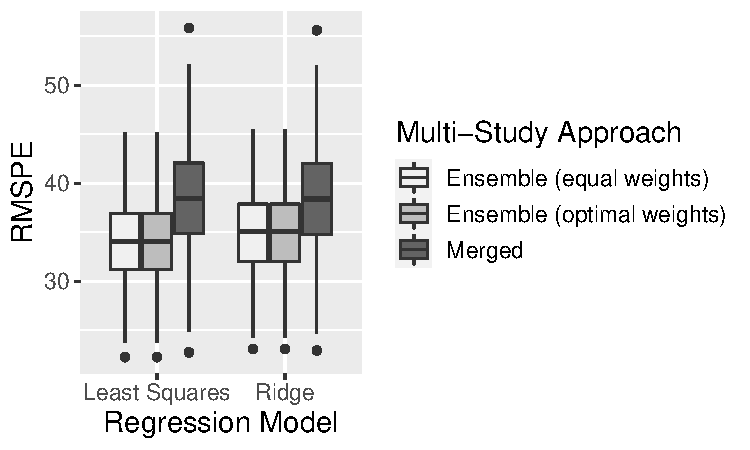
\includegraphics[width=\maxwidth]{figure/unnamed-chunk-15-1} 

}


\begin{kframe}\begin{alltt}
\hlcom{# save figure}
\hlkwd{library}\hlstd{(gridExtra)}
\hlkwd{png}\hlstd{(}\hlstr{'rmse_scenario1.png'}\hlstd{,} \hlkwc{width}\hlstd{=}\hlnum{800}\hlstd{,} \hlkwc{height}\hlstd{=}\hlnum{500}\hlstd{,} \hlkwc{res}\hlstd{=}\hlnum{100}\hlstd{)}
\hlkwd{ggplot}\hlstd{(err2,} \hlkwd{aes}\hlstd{(`Regression Model`, RMSPE,} \hlkwc{fill}\hlstd{=`Multi-Study Approach`))} \hlopt{+} \hlkwd{geom_boxplot}\hlstd{()} \hlopt{+} \hlkwd{theme}\hlstd{(}\hlkwc{text} \hlstd{=} \hlkwd{element_text}\hlstd{(}\hlkwc{size} \hlstd{=} \hlnum{14}\hlstd{))} \hlopt{+} \hlkwd{scale_fill_brewer}\hlstd{(}\hlkwc{palette}\hlstd{=}\hlstr{"Greys"}\hlstd{)}
\hlkwd{dev.off}\hlstd{()}
\end{alltt}
\begin{verbatim}
## pdf 
##   2
\end{verbatim}
\end{kframe}
\end{knitrout}


\end{document}
